\documentclass{article}
\usepackage[utf8]{inputenc}

\usepackage{pifont}
\usepackage{amsfonts}
\usepackage{enumitem}
\usepackage{amssymb}
\newlist{todolist}{itemize}{2}
\setlist[todolist]{label=$\square$}
\newcommand{\cmark}{\ding{51}}%
\newcommand{\xmark}{\ding{55}}%
\newcommand{\done}{\rlap{$\square$}{\raisebox{2pt}{\large\hspace{1pt}\cmark}}%
	\hspace{-2.5pt}}

\title{Synthesizing emotive art}
\author{Konrad Cybulski}
\date{March 2019}

\usepackage{natbib}
\usepackage{graphicx}

\begin{document}
	
\maketitle


\section{Introduction}

In the domain of creative artificial intelligence and evolutionary art, the desire exists for processes that produce imagery that is not only visually appealing, but images that exhibit abstract and emotive characteristics.
There exists extensive research on the production of realistic, and target label accurate images.
The use of quality-diverse (QD) algorithms in combination with deep neural network (DNN) image classifiers were used by \citet{nguyen2015innovation} to generate images with high classification accuracy from pre-trained DNN.
\citet{bao2017cvae} exmplifies recent use of variational generative adversarial network (GAN) architectures for the generation of realistic images from fine-grained target labels.
GANs have shown their use in text-to-image synthesis \citep{reed2016generative, zhang2017stackgan}, producing realistic images reflecting the detailed description from which they are generated.
With regard to creative image generation, \citet{tan2017artgan} explored techniques for synthesizing artwork with more abstract characteristics.
Through the use of a target artist or genre, the generative network produced images that were highly abstract and stylistically accurate.

Little exploration however has been done on incorporating emotion into the process of art and image generation.
\citet{ali2017emotional} explored the idea of \textit{emotion transfer}, using techniques such as image emotion assignment, and color/style transfer with the aim of altering image composition to reach a target emotion.
Examples given use a target profile, with varying levels of emotions such as joy, anger, and fear, to alter the image's color composition.
The classification of an image's affective emotion, the emotion with which a viewer classifies the image, has been explored in various works \citep{machajdik2010affective, chen2015learning, kim2018building}.
\citet{kim2018building} produced a classifier for recognizing the emotion attributed to an image.
This was done through the application of a DNN to decompose an image to a two-dimensional feature vector (valence and arousal) representing the image's emotion mapped to a continuous plane (see Figure \ref{fig:valence-arousal}).


\section{Aims}

The aim of this research is to explore the synthesis of artwork with a target emotional profile.
Primarily leveraging work by \citet{tan2017artgan} and \citet{kim2018building} to produce a generative architecture whose output not only has desirable abstract characteristics, but shows emotive capabilities.
The proposed system would generate an image that satisfies a set of emotions provided.
This will investigate both the efficacy with which a generative system can create emotive images, as well as give insight into the properties attributed to various emotions portrayed in image form.

In order to test, and verify the output of such a system, generated images will be exhibited to explore their emotional effect on humans, and any dissonance between the intended, and resulting emotional profile.
This will further verify the accuracy with which an emotional profile can be synthesized into affective artwork with such an architecture.


\section{Background}

\subsection{Unsupervised image synthesis}
\begin{todolist}
	\item Image generation methods explored: evolutionary algorithms, neural networks, line drawing, etc.
	\item Measuring \textit{goodness} of a generated image: realism, abstractness, aesthetic appeal, etc.
\end{todolist}

\begin{figure}[h!]
	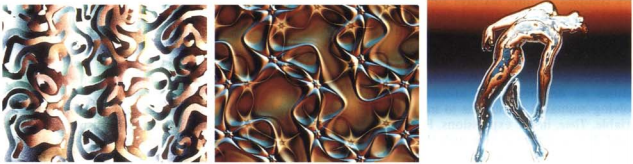
\includegraphics[width=\textwidth]{images/sims-interactive-image-generation.png}
	\caption{Images generated through the process of interactive evolution introduced by \citet{sims}}
	\label{fig:sims}
\end{figure}

The area of evolutionary art and image generation has been explored for many years.
Some of the first \textit{human-in-the-loop} systems such as \textit{NEvAr} \citep{nevar} produced greatly impressive images leveraging methods introduced and exemplified by \citet{sims} such as those shown in Figure \ref{fig:sims}.
\citet{sims} proposed using \textit{Lisp} expressions for genotype definitions, which accepted a coordinate (x, y) which could be evaluated into a grayscale or RGB value, thus producing images.
This genotype expression has been used in numerous further research into the process of both supervised and unsupervised image synthesis \citep{nevar, sims, den2011evolving, distributed-evolutionary-art, aesthetic-measures}.

\citet{sims} and \citet{nevar} were able to produce images with visually striking characteristics, despite the slow nature of the interactive process.
\citet{aesthetic-measures} investigated the use of measures of aesthetics for fitness evaluation in artificially evolving images.
This research primarily used the observation of \citet{ralph-bell-curve}, that the distribution of colour gradients in fine art tend towards normal.
While the images produced through this method did not meet the level of intricacy and detail as the results of \citet{sims} or \citet{nevar}, it represented a self-contained system able to generate appealing art without human interaction.

Introduction of the generative adversarial network architecture (GAN) by \citet{GAN} allowed the process of image generation to be completely unsupervised.
Common GAN application has involved the generation of realistic images, such as has been done by \citet{bao2017cvae}, where images have been synthesized to fine-detailed target labels such as bird species' and actors.
\citet{zhang2017stackgan} and \citet{reed2016generative} have recently explored text to image synthesis, in which detailed descriptions of birds and flowers have been converted into photo-realistic images using the GAN model.
\citet{tan2017artgan} has explored the generation of art according to target genre and artist.

\subsection{Generative adversarial networks}
\begin{todolist}
	\item What is the generative adversarial network, and differences in common architectures
	\item Why are GANs advantageous over the use of target feature analysis (aesthetics, etc.)
	\item Text-to-image
	\item Style transfer \& image-to-image
\end{todolist}

Deep neural networks (DNN) have grown tremendously in popularity within the domain of image generation, and classification.

	
\subsection{Image emotion recognition}
\begin{todolist}
	\item Sentiment classification: text \& images.
	\item Emotion classification in images: facial expression, general imagery.
	\item Methods of classifying emotion in images: single target emotion, discrete categorical likelihood, decomposition into continuous vector (valence-arousal).
\end{todolist}
	
\begin{figure}[h!]
	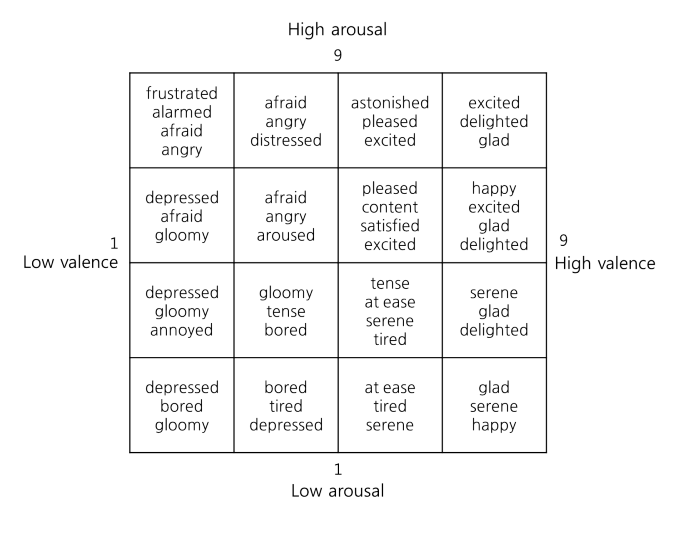
\includegraphics[width=0.75\textwidth]{images/valence-arousal-grid.png}
	\caption{Distribution of emotions associated with levels of valence and arousal determined by DNN classifier produced by \citet{kim2018building}}
	\label{fig:valence-arousal}
\end{figure}

The area of image emotion and sentiment classification has been explored in a number of ways, primarily through image feature analysis derived from art and psychological factors \citep{machajdik2010affective}; and more recently using techniques such as deep neural networks \citep{chen2015learning, kim2018building}.
Feature extraction and analysis has been used for various applications such as measuring aesthetic appeal \citep{den2010using,den2010comparing,den2011evolving} and as an emotional feature vector for sentiment classification \citep{machajdik2010affective}.
Due to the artistic and psychological underpinnings used by \citet{machajdik2010affective}, the low-level features extracted from images can be understood at a high level.
The relationship between an image's emotion and its core artistic components such as balance, harmony, and variety was further explored by \citet{zhao2014exploring}, which uses a comparably small feature vector to \citet{machajdik2010affective}, resulting however in a 5\% classification increase to state-of-the-art approaches at the time.

Deep neural networks in this domain provide less transparency to the process with which emotions and sentiment are classified compared to feature analysis.
The emotional content of an image can be decomposed in various ways.
Image databases with singular emotion labels, and adjective-noun pairs (ANP) have been used for the training of deep neural network classifiers \citep{chen2014deepsentibank, yang2018visual} with up to 200\% performance gains over support vector machine classifiers.


\section{Methodology}

\begin{todolist}
	\item Emotion profile representation
	\begin{todolist}
		\item Discrete feature vector
		\item Continuous valence-arousal space
	\end{todolist}
	\item System architecture (training/evaluation method)
	\begin{todolist}
		\item Generator: input type (related to emotion profile representation)
		\item Generator: base architecture e.g. use ArtGAN \citep{tan2017artgan}
		\item Discriminator: use output image's emotion classification and error from target emotional profile as error function (autoencoder method)
		\item Discriminator: use image label as target emotional profile and use standard logistic discrimination.
	\end{todolist}
	\item Any interaction made between human and generator e.g. text-to-image synthesis using text emotion classification fed through to the generative model.
	
\end{todolist}


\section{Expected Outcomes \& Contributions}

The outcomes of this project will include a generative system with which art can be synthesized according to a target emotional profile.
This system will be the combination of methods for the representation of emotion for use in a generative model, and an architecture with which such a model can be trained.
Due to the exploratory nature of the project with respect to both system architecture and emotional profile representation, this research will have tested and analyzed various options and any comparative differences.

The proposed generative system will be used to create a collection of art, categorised by the target emotional profile with which they were seeded.
The verification proposed involves the public exhibition of produced images, providing feedback to the generative process and pairing the generated images with a human assigned emotion label for use in any further system training.


\bibliographystyle{apalike}
\bibliography{references}

\end{document}
